%!TEX TS-program = xelatex
%!TEX encoding = UTF-8 Unicode
\documentclass[11.5pt]{beamer}
%\usepackage{pgfpages}
%\pgfpagesuselayout{4 on 1}[a4paper,border shrink=5mm]

\usepackage[english]{babel}
%\usepackage[utf8x]{inputenc}

% mathmatical fonts and formulations
\usepackage{amsfonts}
\usepackage{amsmath}
\usepackage{amsthm}
\usepackage{amssymb}
% float control
\usepackage{placeins}
% graphic control
\usepackage{pgf}
\usepackage{tikz}
\usepackage{xcolor}
% Algorithm support
%\usepackage{algorithmic}
\usepackage{algorithm2e}
%color of the word
\usepackage{color}
% change the counter of enumerate
\usepackage{enumerate}
\usepackage{fix-cm}

\usepackage{mathspec}


%\usepackage{fontspec,xltxtra,xunicode}
\defaultfontfeatures{Mapping=tex-text}
%\setsansfont[Scale=MatchLowercase,Mapping=tex-text]{Comic Sans MS}

%\setmathsfont(Digits,Latin,Greek)[Numbers={Lining,Proportional}]{Comic Sans MS}

\mode<presentation>
{
  \usetheme{default}      % or try Darmstadt, Madrid, Warsaw, ...
  \usecolortheme{default} % or try albatross, beaver, crane, ...
  \usefonttheme{default}  % or try serif, structurebold, ...
  \setbeamertemplate{navigation symbols}{}
  \setbeamertemplate{caption}[numbered]
  \setbeamertemplate{footline}[frame number]
} 
\setbeamertemplate{frametitle}{
	\vspace{1em}
	\begin{center}{
	\Huge{\insertframetitle}
	}
	\end{center}
}



\title{COMP 3721}
\author{Tutorial 5}
%\institute{}
%\date{\today}

\begin{document}

\begin{frame}
  \titlepage
\end{frame}

\begin{frame}[t]
\frametitle{Context-Free Grammar}
\begin{enumerate}[(1)]
\item Show that the following languages are context-free by exhibiting context-free grammars generating each.
    \begin{enumerate}[(a)]
        \item<1-> $\{\text{$w\in \{a,b\}^*$ : $w = w^R$}\}$
        \only<2>{
            \begin{itemize}
                \item $V = \{a,b,S\}$
                \item $\Sigma = \{a,b\}$
                \item $R = \{S\to aSa, S\to bSb, S\to e, S\to a, S\to b\}$
            \end{itemize}
        }
        \item<3-> $\{\text{$a^mb^n$ : $m\geq n\geq 0$}\}$
        \only<4>{
            \begin{itemize}
                \item $V = \{a,b,S\}$
                \item $\Sigma = \{a,b\}$
                \item $R = \{S\to e, S\to aSb, S\to aS\}$
            \end{itemize}
        }
        \item<5-> $\{\text{$a^mb^nc^pd^q$ : $m+n = p+q$}\}$
        \only<6>{
            \begin{itemize}
                \item $V = \{a,b,c,d,A,B,X,S\}$
                \item $\Sigma = \{a,b,c,d\}$
                \item $R = \{S\to aSd, S\to A, S\to B, A\to aAc, A\to X, B\to bBd, B\to X, X\to bXc, X\to e\}$
            \end{itemize}
        }
    \end{enumerate}
\end{enumerate}
\end{frame}

\begin{frame}[t]
\frametitle{Context-Free Grammar}
\begin{enumerate}[(2)]
\item Let $G = (V,\Sigma,R, S)$, where $V = \{a, b, S\}$, $\Sigma = \{a, b\}$, and $R = \{S \to aSb, S \to aSa, S \to bSa, S \to bSb, S \to e\}$. Show that $L(G) = \{\text{$w \in \{a, b\}^*$ : $w$ has even length}\}$.
\end{enumerate}
\end{frame}

\begin{frame}[t]
\frametitle{Proof}
\begin{itemize}
\item It is easy to see that any string generated by $G$ have even length since every rule of $G$ generates even number of terminals.

\item Now it suffices to show that any string $w$ of even length can be generated by $G$. We prove this by induction on the length of $w$. 
\begin{enumerate}[(i)]
\item When $|w| = 0$, it is obvious that $w$ can be generated by $G$. 
\item Suppose that when $|w| = 2i$, $w$ can be generated by $G$. 
\item We show that when $w = 2(i+1)$, $w$ can be generated by $G$. Suppose $w$ starts with $a$ and ends with $a$ (the other three cases can be handled in a similar way). Then $w = aya$ for some $y$ with $|y| = 2i$. By the inductive hypothesis, $w$ can be generated as follows.
    \begin{displaymath}
        S \Rightarrow aSa \Rightarrow^* aya = w
    \end{displaymath}
\end{enumerate}
\end{itemize}
\end{frame}

\begin{frame}[t]
	\frametitle{Pushdown Automata}
	\begin{enumerate}[(1)]
		\item Construct a pushdown automaton that accepts the language $\{\text{$a^ib^j$ : $i \leq 2j$}\}$.
		
		\vspace{2em}
		\uncover<2>{
			Solution: 
			\begin{center}
				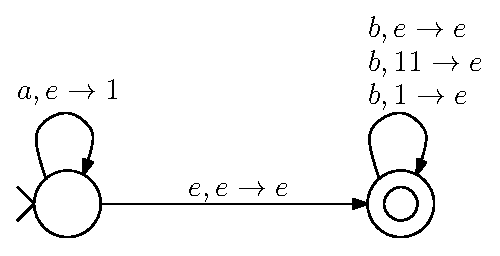
\includegraphics[scale = 0.6]{q1.eps}
			\end{center}
		}
	\end{enumerate}
\end{frame}

\begin{frame}[t]
	\frametitle{Pushdown Automata}
	\begin{enumerate}[(2)]
		\item Construct a pushdown automaton that accepts the language $\{\text{$a^ib^jc^k$ : $i = j + k$}\}$.
		
		\vspace{2em}
		\uncover<2>{
			Solution: 
			\begin{center}
				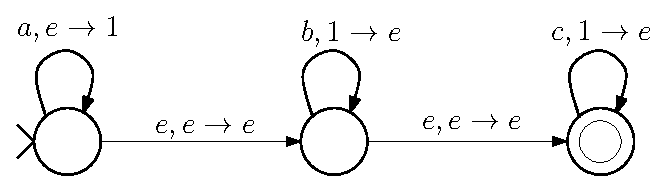
\includegraphics[scale = 0.6]{q2.eps}
			\end{center}
		}
	\end{enumerate}
\end{frame}

\begin{frame}[t]
	\frametitle{Pushdown Automata}
	\begin{enumerate}[(3)]
		\item Construct a pushdown automaton that accepts the following language.
		\begin{displaymath}
			\{\text{$w$ in $\{a, b\}^*$ : $w$ has twice as many $b$'s as $a$'s}\}
		\end{displaymath}
	\end{enumerate}
\end{frame}

\begin{frame}[t]
	\frametitle{Solution}
	\begin{center}
		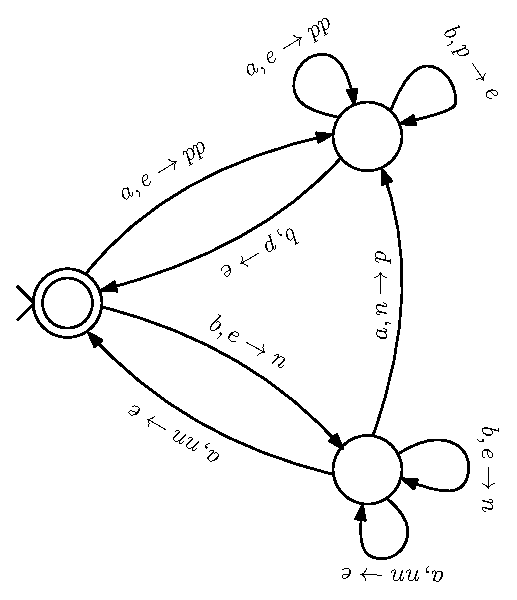
\includegraphics[scale = 0.6]{q3.eps}
	\end{center}
\end{frame}
\end{document}
